\subsection{Analytically solvable settings exist}
\label{sec:reason-dynamics}

A reliable way to build scientific understanding in complex systems is to study pared-down yet representative settings in which quantitative calculations are possible.
For example, physics uses representative solvable settings like the harmonic oscillator and the hydrogen atom as sources of intuition for much broader classes of system.
Deep learning appears to be particularly amenable to this approach: scientists have identified a rich landscape of minimal models where the learning dynamics simplify and many quantities of interest become solvable.
These analytically tractable cornerstones are useful because they reveal phenomena and mechanisms to look for when we turn to realistic deep learning.%
\footnote{A complementary view is that any eventual complete theory of deep learning must encompass these simplified settings. Their solutions may provide conceptual scaffolding, serving as nucleation sites from which a more general theory crystallizes.}


One particularly fruitful simplification is \textit{linearization}.
Here we discuss two distinct instantiations of this idea: linearization in the data, where $f(\vx;\vtheta)$ becomes linear in $\vx$, and linearization in the parameters, where $f(\vx;\vtheta)$ becomes linear in $\vtheta$.



\begin{figure}
    \centering
    \begin{subfigure}{0.5\linewidth}
        \centering
        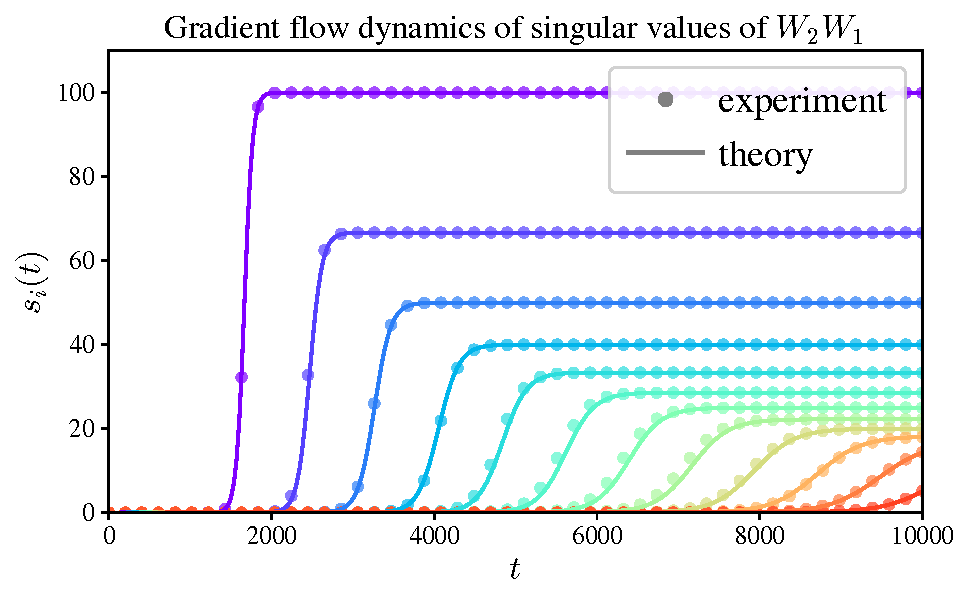
\includegraphics[width=\linewidth]{figs/analytic/mfac_dynamics.pdf}
        \caption{Linearization in the data}
        \label{fig:sub1}
    \end{subfigure}
    \hfill
    \begin{subfigure}{0.48\linewidth}
        \centering
        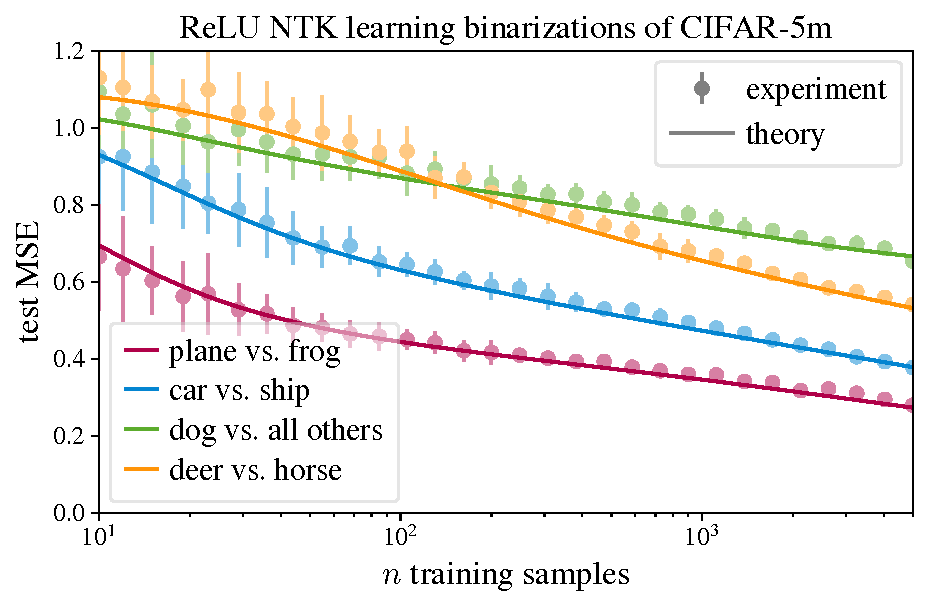
\includegraphics[width=\linewidth]{figs/analytic/ntk_learning_curves.pdf}
        \caption{Linearization in the parameters}
        \label{fig:sub2}
    \end{subfigure}
    \caption{
    \textbf{Linearization yields exact solutions that match experiments.}
    (a) Canonical work by \citet{saxe2014exact} showed that, under a task-aligned initialization $\vtheta^{(0)}$ and whitened inputs $\vx \sim \mathcal{N}(0,\mathbf{I})$, the gradient flow learning dynamics of deep linear networks decouple into independent solvable Bernoulli ODEs.
    This leads to sequential learning of singular modes, with larger-singular-value modes emerging first.
    Panel (a) reproduces Fig.~3 of \citet{saxe2014exact}.
    (b) Linearizing a nonlinear network by truncating nonlinear terms in its Taylor expansion around initialization reduces least-squares training to kernel ridge regression with the neural tangent kernel (NTK).
    This analysis connects the network's architecture to its inductive bias through the NTK eigenstructure, enabling accurate predictions for the test performance of these networks.
    Panel (b) is based on Fig.~2 of \citet{simon2023eigenlearning}.
    }
    \label{fig:linearization}
\end{figure}




\paragraph{Linearization in the data.}
A \emph{deep linear network} is obtained by removing all nonlinearities from a neural network's architecture, yielding a model that is linear in its inputs $\vx$ but remains highly \emph{nonlinear} in its parameters $\vtheta$:
\begin{equation}
    f(\vx;\vtheta) = \mathbf{W}_L \mathbf{W}_{L-1} \cdots \mathbf{W}_1 \vx,
    \qquad
    \text{where }  \vtheta := \{\mathbf{W}_\ell\}_{\ell = 1}^L\text{, each }\mathbf{W}_\ell \text{ is a linear transformation, and } L \ge 2.
\end{equation}
Deep linear networks have a long history of study because, despite their simplicity, they retain many hallmark behaviors of deep learning \citep{nam2025position}. These include saddle-point-dominated loss landscapes \citep{baldi1989neural}, dynamics with sharp phase transitions and separation of timescales \citep{gissin2019implicit,atanasov2021neural}, edge-of-stability oscillations with gradient descent \citep{even2023s}, and strong initialization-dependent inductive biases \citep{woodworth2020kernel, kunin2024get}.
Analysis of these networks is typically carried out with the \emph{gradient flow} learning rule --- the continuous-time limit of gradient descent --- under simplifying assumptions on the data distribution and with carefully chosen initializations \citep{fukumizu1998effect,saxe2014exact,tarmoun2021understanding,domine2025lazy}.
In these regimes, the learning dynamics can often be solved exactly or reduced to low-dimensional dynamical systems.


Across many such analyses, a consistent lesson emerges: learning exhibits a \emph{greedy} low-rank bias, acquiring some components of the task before others.
Canonical work by \citet{saxe2014exact} first showed how deep linear networks learn singular vectors of the input–output correlation sequentially during training, with learning prioritized toward modes associated with the largest singular values, as shown in \cref{fig:linearization}.
This bias has been hypothesized to benefit generalization by separating the signal from the noise \citep{lampinen2018analytic}, and closely mirrors behavior observed in nonlinear networks, where simpler functions are often learned before more complex ones \citep{kalimeris2019sgd, simon2023stepwise}.
Moreover, a range of factors --- including small initializations \citep{gidel2019implicit,li2021towards,jacot2021saddle,pesme2023saddle}, increased depth \citep{gunasekar2018implicit, arora2018optimization, arora2019implicit}, stronger mini-batch noise \citep{pesme2021implicit,chen2024stochastic}, and explicit $\ell_2$ regularization \citep{ziyin2022exact,wang2024implicit} --- have all been shown to further strengthen this greedy learning bias.


\paragraph{Linearization in the parameters.}

A \textit{linearized network} is obtained by truncating the nonlinear terms in a network's Taylor expansion around its initial parameters. This yields a model that is linear in its parameters $\vtheta$ but remains highly \emph{nonlinear} in the data $\vx$:
\begin{equation}
    f_\text{lin}(\vx;\vtheta) = f(\vx;\vtheta_0) + \nabla_{\vtheta} f(\vx;\vtheta_0)^\top (\vtheta-\vtheta_0),
    \qquad
    \text{where } \nabla_{\vtheta} f(\cdot;\vtheta_0)  \text{ is the gradient at initialization.}
\end{equation}
This is not some contrived construction: in fact, there are settings in which a model is well-approximated throughout training by its linearization, i.e., $\forall t,\  f(\vx;\vtheta_t)\approx f_\text{lin}(\vx;\vtheta_t)$.
For example, any neural network architecture can be driven into the linearized regime by taking suitable limits \citep{jacot2018neural,lee2019wide,chizat2019lazy,liu2020linearity}, as discussed in \cref{sec:reason-limits}.
Additionally, recent evidence suggests that language model fine-tuning occurs in a near-linearized regime \citep{malladi2023kernel,ren2025learning}.

Since a linearized network is linear in its parameters, its learning dynamics are identical to those of linear regression, with one key difference:
while the dynamics of linear regression are driven by the Gram kernel, $K_\text{Gram}(\vx,\vx')=\vx^\top\vx'$, linearized networks are described by the \textit{neural tangent kernel} (NTK), $K_\text{NTK}(\vx,\vx')\coloneqq \nabla_{\vtheta} f(\vx;\vtheta_0)^\top \nabla_{\vtheta} f(\vx';\vtheta_0)$.
When the task is least squares regression and training uses small-step gradient descent, the dynamics are analytically tractable and the final predictor is given by kernel ridge regression with the NTK \citep{jacot2018neural}.


This setting yields insight into a variety of deep learning phenomena.
For example, since the details of the network architecture influence the mathematical structure of the NTK through the fixed feature map $\nabla_{\vtheta} f(\cdot;\vtheta_0)$, one learns how the linearized model's inductive bias follows from its architecture \citep{arora2019exact,geifman2020similarity}.
Furthermore, one may accurately predict the model's expected generalization error on arbitrary targets $f^\star$ by accounting for the structure of the input data \citep{jacot:2020-KARE,canatar2021spectral,loureiro:2021-learning-curves,hastie:2022-surprises,wei2022more,simon2023eigenlearning}, as shown in \cref{fig:linearization}.
Applying this framework to realistic data distributions uncovers the origin of the typical models' tendency to learn simple and generalizing functions \citep{basri2020frequency,karkada2025predicting}.
Linearized models also capture relevant phenomena such as double descent \citep{belkin2019reconciling, advani2020high} and scaling laws \citep{caponnetto2007optimal,pillaud2018statistical, cui2023error, atanasov2024scaling}.

However, despite these theoretical merits, linearized networks are unrealistic in a few critical ways.
Most notably, they do not capture the strong feature-learning capabilities that generic neural networks exhibit, often leading to overly pessimistic predictions for sample complexity \citep{ghorbani2020neural,vyas2022limitations}.
Moreover, by reducing training to a tractable linear problem, these models sidestep the intrinsically nonconvex optimization phenomena of deep learning.
To describe these and other aspects of deep learning, one must look beyond linearization.

\paragraph{Beyond linearization.}
An important frontier for theory lies in developing analytically tractable toy models that remain genuinely nonlinear in both the data and the parameters (see \cref{openquestion:models_of_nonlin_learning}).
In these settings, the influence of the data distribution becomes more complex, making it difficult to obtain a unified and general framework.
However, a growing body of work is progressing in this direction by isolating specific nonlinear mechanisms and making them solvable under assumptions on the data.

One line of work studies Gaussian inputs and structured targets (e.g., single- and multi-index models). Fully nonlinear neural networks provably outperform kernel methods using fewer samples because they exploit the structure in the target function to learn relevant features \citep{abbe2022merged, damian2022neural, bietti2022learning, ba2022high, dandi2023two}. Complementarily, methods from statistical physics enable computing exact asymptotics for Bayes-optimal inference and learning dynamics in these models \citep{barbier2019optimal, aubin2018committee, mignacco2020dynamical}. A related setting is two-layer neural networks with quadratic activation functions, where recent results have characterized the exact asymptotics, training dynamics, and scaling laws \citep{erba2025nuclear, arous2025learning, defilippis2025scaling, ren2025emergence}. Several other lines of research isolate distinct nonlinear phenomena: the convergence of homogeneous networks trained on logistic losses to max-margin solutions \citep{soudry2018implicit, lyu2020gradient}, the reduction of training dynamics to low-dimensional summary statistics in teacher-student models \citep{saad1995exact, goldt2019dynamics, ben2022high, veiga2022phase, zavatone2025summary}, memorization in associative memory models \citep{nichani2025understanding}, learned algorithmic structure in modular arithmetic tasks \citep{morwani2023feature, gromov2023grokking, kunin2025alternating}, nonlinear solvable models of attention \citep{zhang2025training, boncoraglio2025singlehead},
and improved scaling laws from nonlinear feature learning \citep{bordelon2025feature}.

Taken together, these approaches illustrate both the promise and the limitations of current nonlinear toy models: each captures a slice of fully nonlinear learning dynamics, yet no unified framework has emerged.
We view this space as an open and rapidly evolving area, and return to these challenges in our discussion of open problems in \cref{sec:open_dirs}.
